\documentclass[tikz,border=2pt]{standalone}
\usepackage{amsmath}
\usepackage{pgfplots}
\pgfplotsset{compat=1.18}
\usetikzlibrary{arrows.meta}
\begin{document}
% Exercise 1.26 with delta=5, beta=-4: f=0 for x<0, x^3 on [0,1], 5x-4 for x>1. At the joint 1 the left derivative is 3
% (tangent 3x-2) and the right derivative is 5>=3, so f is convex; delta=1 (beta=0, line x) would drop the slope to 1.
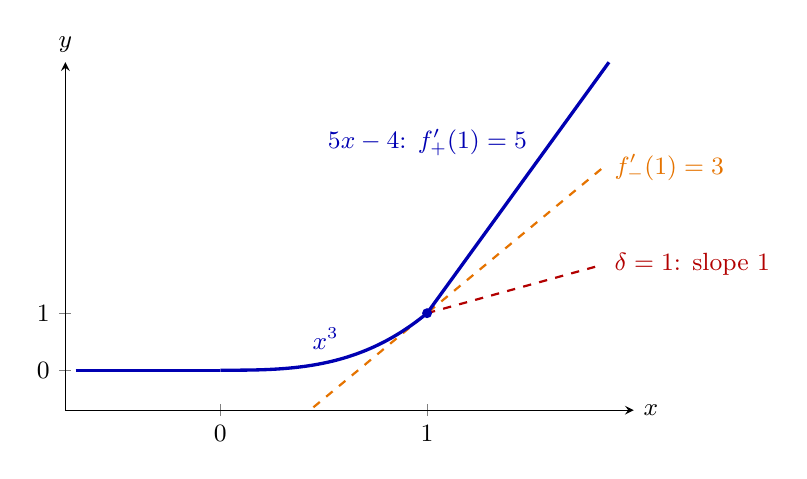
\begin{tikzpicture}[font=\small, >={Latex[length=2mm]}]
  \begin{axis}[
    axis lines=left, xmin=-0.75, xmax=2.0, ymin=-0.7, ymax=5.4,
    xtick={0,1}, ytick={0,1},
    xlabel={$x$}, ylabel={$y$},
    xlabel style={at={(axis description cs:1,0)}, anchor=west},
    ylabel style={rotate=-90, at={(axis description cs:0,1)}, anchor=south},
    width=8.8cm, height=6cm, clip=false
    ]
    \draw[orange!90!black, thick, dashed] (axis cs:0.45,-0.65) -- (axis cs:1.85,3.55);
    \addplot[red!70!black, thick, dashed, domain=1:1.85, samples=2] {x};
    \addplot[blue!70!black, very thick] coordinates {(-0.7,0) (0,0)};
    \addplot[blue!70!black, very thick, domain=0:1, samples=60] {x^3};
    \addplot[blue!70!black, very thick, domain=1:1.88, samples=2] {5*x-4};
    \fill[blue!70!black] (axis cs:1,1) circle (1.8pt);
    \node[blue!70!black, anchor=east] at (axis cs:0.62,0.55) {$x^3$};
    \node[blue!70!black, anchor=east] at (axis cs:1.53,4.0) {$5x-4$: $f'_{+}(1)=5$};
    \node[orange!90!black, anchor=west] at (axis cs:1.86,3.55) {$f'_{-}(1)=3$};
    \node[red!70!black, anchor=west] at (axis cs:1.86,1.85) {$\delta=1$: slope $1$};
  \end{axis}
\end{tikzpicture}
\end{document}
